\chapter{Graph segmentation}
\label{chap:track-building}

Given a set of scored edges, the last stage of the pipeline segments them into individual track candidates. 
There are several methods to carry out this task. 
The simplest case applies a score threshold to eliminate edges believed to be faked, and treats the remaining connected subgraphs as track candidates. 
This approach, called \textbf{Connected Component}, ignores the directionality of graph edges.
At the other edge of complexity, the edge direction is retained and exploited to make heuristic segmentation decisions. 
A subgraph is traversed outward from a source node--one with no incoming edges, selecting the longest path to form a track candidate.
This method is called \textbf{Walkthrough}. 
Both approaches are detailed in this chapter, starting with the simple Connected Component.
The track candidates constructed by the Walkthrough algorithm are used to evaluate tracking performance in chapter \ref{chap:tracking-performance}.

\section{Connected components}
\label{sect:cc}
The simplest and most intuitive method of track building involves pruning the graph of edges that are deemed fake.
Assigned to each edge by the GNN is a score $s\in [0,1]$ representing the probability that it is a true edge. 
A binary label is obtained from a threshold $s_{cut}$, which reflects the level of confidence one desires in a prediction of a positive edge
\beq
\label{eq:11.1}
\hat{y}_{ij} = \mathds{1}_{s_{ij} > s_{cut}}.
\eeq
The threshold is typically set to $s_{cut}=0.5$ in typical classification problems.
However, the score cut in our problem needs not follow this convention.
Figure \ref{fig:gnn-edge-score} shows the score distribution of the GNN on graphs constructed with Metric Learning method, categorized by the true label.
We observe an excellent separation between target and fake edges. 
$99.6\%$ of fake edges have score lower than 0.01, with the highest among other bins contributing $<0.1\%$. 
On the other hand, $99.7\%$ of target edges get score higher than 0.01. 
This means that even a loose $s_{cut}=0.01$ eliminates $99.6\%$ fake edges and retains $99.7\%$ target edges. 
The edge efficiency and fake reduction of several other cuts are shown in table \ref{tab:score-cuts}.
It is obvious that the edge efficiency decreases, while the fake reduction increases with tightening score cut.
It is also clear that for our purpose, we lose too much efficiency at $s_{cut}=0.5$, making it sub-optimal. 
A score cut of $s_{cut}=0.01$ is chosen to label the graph edges. 
\begin{figure}[h!]
    \centering
    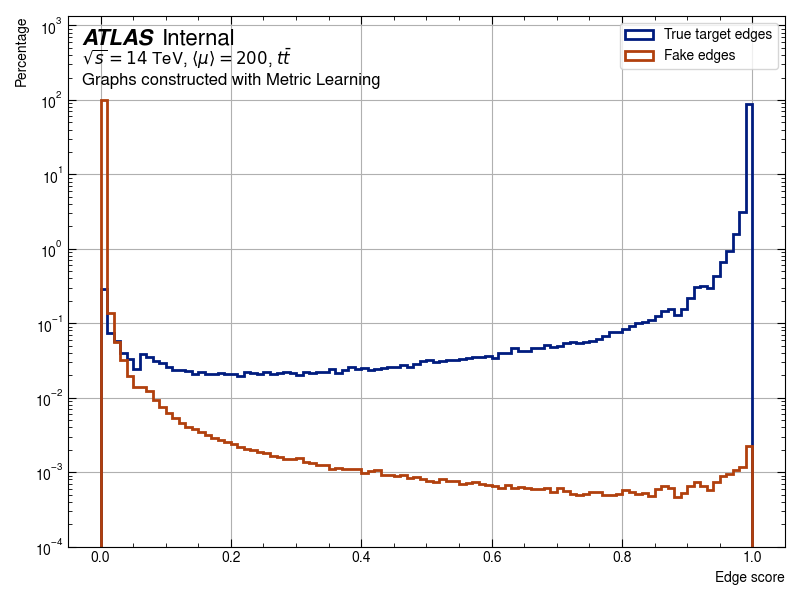
\includegraphics[width=0.65\textwidth]{figures/gnn/gnn-edge-score.png}
    \caption{A distribution of the GNN edge classification scores. 200 graphs constructed using the Metric Learning approach are used.}
    \label{fig:gnn-edge-score}
\end{figure}

Illustrated in figure \ref{fig:connected-component}, the elimination of fake edges results in the segmentation of the input graph into subgraphs which are not connected to the rest of the graph. Mathematically, the segmented graph can be written as
\beq
\label{eq:11.2}
G(V,E)=\bigcup_{i=1}^{M} G(V_i, E_i)
\eeq
where for any pair $i\neq j,\,i\in [M], \, j\in[M]$, 
\beq
\label{eq:11.3}
V_i \cap V_j = \varnothing, \quad E_i \cap E_j = \varnothing 
\eeq
figure \ref{subfig:gnn-input-graph}, shows a simplified input graph to the GNN, which contains two color-coded tracks: a \textbf{\textcolor{SeaGreen}{green}} track with 4 hits labelled $\{1,2,3,4\}$, a \textbf{\textcolor{RoyalBlue}{blue}} track with 3 hits labelled $\{5,6,7\}$; and a single \textbf{\textcolor{Plum}{violet}} hit labelled $\{8\}$. 
Hits and true edges from a track share the same color. 
Fake edges are shown in \textbf{\textcolor{BrickRed}{red}}. 
Note that the colours represent truth information available only for evaluation. 
During inference, the GNN \textbf{ideally} gives \textbf{\textcolor{BrickRed}{fake}} edges a low score, and true edges a high score. 
After eliminating edges whose score falls belows $s_{cut} = 0.01$, we are left with three correctly segmented subgraphs, each containing all hits from the parent particle. 
Every node in each subgraph has at most 1 incoming and 1 outgoing edge, creating a single path from the innermost to the outermost hit \footnote{Note that all input edges point in the direction of increasing distance from the IP}. 
These graphs, designated simply connected components, are labelled as track candidates.

\begin{table}[h!]
    \centering
    \begin{tabular}{c|c|c}
       Score cut  & Edge efficiency [\%] & Fake reduction [\%] \\ \hline \hline
        0.01         & 99.71  &  99.58 \\
        0.02 & 99.63 & 99.72 \\
        0.05 & 99.50 & 99.82  \\
         0.1 & 99.35 & 99.89 \\
        0.2 & 99.12 & 99.93 \\
        0.5 & 98.42 & 99.97 \\ 
        \hline
    \end{tabular}
    \caption{Edge efficiency and fake reduction rate at representative values of GNN edge score cut. }
    \label{tab:score-cuts}
\end{table}

Because of its simplicity, \textbf{Connected Component} is fast and widely available in many Python libraries. 
We use the \textsc{NetworkX} library\cite{NetworkX} to implement the segmentation, which has a GPU backend called \textsc{Nx-Cugraph}.
The latter allows the GNN-labelled graph which already resides on the GPU during inference to be segmented without being moved to the CPU, avoiding data transfer overheads. 

\begin{figure}[h!]
\begin{subfigure}[b]{0.32\textwidth}
\centering
    \begin{tikzpicture}[
    roundnode/.style={circle, text=SeaGreen, draw=SeaGreen!100, fill=SeaGreen!10, very thick, minimum size=7mm},
    % every edge quotes/.style = {midway, opacity=1}
    ]
    \node[roundnode] (1) at (0,0) {$1$};
    \node[roundnode] (2) at (-0.5,2) {$2$};

    \node[roundnode] (3) at (-0.2,4.3) {$3$};
    \node[roundnode] (4) at (0.6,6.3) {$4$};
    \node[roundnode, text=RoyalBlue, fill=RoyalBlue!10, draw=RoyalBlue!100, opacity=1] (7) at (-2.1, 4.5) {$7$};
    \node[roundnode, text=RoyalBlue, fill=RoyalBlue!10, draw=RoyalBlue!100, opacity=1] (6) at (-2, 2.3) {$6$};
    \node[roundnode, text=RoyalBlue, fill=RoyalBlue!10, draw=RoyalBlue!100, opacity=1] (5) at (-2.2, 0) {$5$};
    \node[roundnode, text=Plum, fill=Plum!10, draw=Plum!100, opacity=1] (8) at (1.4, 3) {$8$};

    \draw[SeaGreen, very thick, -Stealth] 
    (1) edge (2)
    (2) edge (3)
    (3) edge (4);
    
    \draw[RoyalBlue, very thick, -Stealth,  opacity=1] 
    (5) edge (6)
    (6) edge (7);

    \draw[BrickRed, very thick, -Stealth]
    (2) edge (8)
    (2) edge (6);
    
    \end{tikzpicture}
    \vspace{0.5cm}
    \caption{GNN input graph}
    \label{subfig:gnn-input-graph}
\end{subfigure}
\begin{subfigure}[b]{0.33\textwidth}
\centering
    \begin{tikzpicture}[
        roundnode/.style={circle, text=SeaGreen, draw=SeaGreen!100, fill=SeaGreen!10, very thick, minimum size=7mm},
        % every edge quotes/.style = {midway, font=\small, opacity=1}
    ]
    \node[roundnode] (1) at (0,0) {$1$};
    \node[roundnode] (2) at (-0.5,2) {$2$};

    \node[roundnode] (3) at (-0.2,4.3) {$3$};
    \node[roundnode] (4) at (0.6,6.3) {$4$};
    \node[roundnode, text=RoyalBlue, fill=RoyalBlue!10, draw=RoyalBlue!100, opacity=1] (7) at (-2.1, 4.5) {$7$};
    \node[roundnode, text=RoyalBlue, fill=RoyalBlue!10, draw=RoyalBlue!100, opacity=1] (6) at (-2, 2.3) {$6$};
    \node[roundnode, text=RoyalBlue, fill=RoyalBlue!10, draw=RoyalBlue!100, opacity=1] (5) at (-2.2, 0) {$5$};
    \node[roundnode, text=Plum, fill=Plum!10, draw=Plum!100, opacity=1] (8) at (1.4, 3) {$8$};

    \draw[SeaGreen, very thick, -Stealth] 
    (1) -- (2) node [midway,left=1pt] {0.92};
    \draw[SeaGreen, very thick, -Stealth] 
    (2) -- (3) node [midway,left=1pt] {0.95};
    \draw[SeaGreen, very thick, -Stealth] 
    (3) -- (4) node [midway,left=1pt] {0.87};
    
    \draw[RoyalBlue, very thick, -Stealth,  opacity=1] 
    (5) -- (6) node [midway,left=1pt] {0.93};
    \draw[RoyalBlue, very thick, -Stealth,  opacity=1] 
    (6) -- (7) node [midway,left=1pt] {0.89};
    
    \draw[BrickRed, very thick, -Stealth, opacity=0.2] 
    (2) -- (8) node [midway, text centered, above=1pt,sloped, opacity=1] {0.005};
    \draw[BrickRed, very thick, -Stealth, opacity=0.2] 
    (2) -- (6) node [midway, text centered, above=1pt,sloped, opacity=1] {0.002};
    
    \end{tikzpicture}
    \vspace{0.5cm}
    \caption{Labeled graph}
    \label{subfig:gnn-labeled-graph}
\end{subfigure}
\begin{subfigure}[b]{0.33\textwidth}
\centering
    \begin{tikzpicture}[
    roundnode/.style={circle, text=SeaGreen, draw=SeaGreen!100, fill=SeaGreen!10, very thick, minimum size=7mm},
    % every edge quotes/.style = {midway, opacity=1}
    ]
    \node[roundnode] (1) at (0,0) {$1$};
    \node[roundnode] (2) at (-0.5,2) {$2$};

    \node[roundnode] (3) at (-0.2,4.3) {$3$};
    \node[roundnode] (4) at (0.6,6.3) {$4$};
    \node[roundnode, text=RoyalBlue, fill=RoyalBlue!10, draw=RoyalBlue!100, opacity=1] (7) at (-2.1, 4.5) {$7$};
    \node[roundnode, text=RoyalBlue, fill=RoyalBlue!10, draw=RoyalBlue!100, opacity=1] (6) at (-2, 2.3) {$6$};
    \node[roundnode, text=RoyalBlue, fill=RoyalBlue!10, draw=RoyalBlue!100, opacity=1] (5) at (-2.2, 0) {$5$};
    \node[roundnode, text=Plum, fill=Plum!10, draw=Plum!100, opacity=1] (8) at (1.4, 3) {$8$};

    \draw[SeaGreen, very thick, -Stealth] 
    (1) edge (2)
    (3) edge (4)
    (2) edge (3);

    \draw[RoyalBlue, very thick, -Stealth]
    (5) edge (6)
    (6) edge (7);
    
    \end{tikzpicture}
    \vspace{0.5cm}
    \caption{Segmented graph}
    \label{subfig:gnn-segmented-graph}
\end{subfigure}
\caption{Illustration of the Connected Component method. (a) The input graph contains two particle tracks and a single hits, all color-coded. The three objects are merged by two fake edges in red. (b) Edges whose score falls under a threshold is eliminated. (c) The remaining connected components are considered as track candidates. }
\label{fig:connected-component}
\end{figure}

It is perhaps not surprising that connected component alone is not sufficient to build track candidates with sufficient reconstruction efficiency, which is why its description emphasizes on an ideal GNN labelling.
We already see from figure \ref{fig:gnn-edge-score} that this is not the case. 
Aside from the inefficiency associated with the rejection of true edges with $\hat{y}<0.01$, $0.42\%$ of the fake edges still remain after the edge cut. 
Despite their small population, residual fake edges create a non-negligible number of non-simple subgraphs, with whom the method is not equipped to deal.
These non-simple subgraphs occur then true tracks are merged by a misclassified fake edge, creating an object that fails to represent any of the underlying particle.
We will examine this problem in greater details and its treatment in the next section.

\section{The Walkthrough algorithm}
\label{sect:walk}

Non-simple subgraphs are a big drawback of the Connected Component approach. 
Their topology can range from a random hit being wrongly connected to an otherwise good track, to several tracks being merged together. 
With the only tuneable parameter being the GNN edge score cut, it undergoes a trade-off between the edge efficiency and the fake edge rate. 
A high score cut decreases the efficiency but also the number of fake edges, thus reducing the occurrence of non-simple subgraphs. 
This edge efficiency reduction, however, often results in strong impact on the tracking efficiency of high-$\pT$ particles due to their small proportion. 
To avoid compromising high-$\pT$ tracks, we must contend with a loose score cut and resolve the ensuing merged tracks.

The Walkthrough algorithm is constructed as a solution to this issue.
It still relies on the Connected Component method to quickly construct simple track candidates.
On non-simple subgraphs, however, it considers both the directionality and the GNN edge score to isolate merged tracks. 
The main idea is to traverse all possible paths starting from the source nodes and to identify the longest paths which do not share any node with each other. 
The edge score is used to resolve ambiguity when multiple paths have the same lengths, and other subtle cases.

First, all cycles in the form $u\rightarrow\dotsc \rightarrow v \rightarrow \dotsc \rightarrow u $ are removed.
Although by construction graph edges always point in the direction of increasing distance from the interaction point, a loop can occur when three or more equidistant nodes are connected in a manner such as $v_1\rightarrow v_2\rightarrow v_3 \rightarrow v_1$, in which case one of the edge is randomly flipped to remove the loop. 
The removal of loops enables a topological sort $f: V\rightarrow \mathbb{N}$ of nodes in the subgraph, such that for every directed edge $u\rightarrow v$, $f(u)<f(v)$. 
The sorting places all nodes that have no incoming edges at the top, which are isolated into a set of starting nodes. 
Thanks to the loop removal and the edge orientation, this set is guaranteed non-empty.
Each starting node becomes a seed for iterative track building.

Space points are sequentially added to the seed path, guided by the GNN edge score.
Two thresholds on edge score are defined.
The first, denoted $s_{min}$, is the minimum score of an edge via which the path may be extended.
The second, denoted $s_{add}$ and always larger than $s_{min}$, is the minimum score to create an alternative path.
With these thresholds, three distinct scenarios can be identified.
\begin{enumerate}
    \item A unique outgoing edge exists from the starting node. This is the trivial case. The receiving node is added to the path and becomes the next starting node (figure \ref{subfig:walk-single-branch}),
    \item Multiple outgoing edges stem from the starting node, among which the highest score $s_{max} \le s_{add}$. The edge with the highest score is uniquely chosen and its receiving node becomes the next starting node (figure \ref{subfig:walk-three-branch-admit-one}),
    \item Multiple outgoing edges stem from the starting node, and $s_{max} \ge s_{add}$. All edges with $s>s_{add}$ are admitted to create multiple parallel paths, each now starting from the corresponding receiving node (figure \ref{subfig:walk-three-branch-admit-two}).
\end{enumerate}
In these scenarios, the scores of all considered edges must exceed $s_{min}$.
This local procedure is repeated until all paths reach a terminal node, from which no outgoing edge stems.
In the end, every encounter of scenario (3) creates at least two track paths. 
To resolve the ambiguity, we select the longest path. 
Thus, from a given starting node, we obtain a single track candidate, whose node are removed from the parent subgraph.
This prevents space points from being shared among multiple track candidates.
Nodes from the globally rejected paths, and locally rejected nodes can be reused to build track candidates from other starting nodes.

% If from the starting node exists a unique outgoing edge with $s>s_{min}$, the space point at its receiving end (the receiver) is added to the path and becomes the next starting node . 
% If multiple possible paths exist,  (figure \ref{subfig:walk-three-branch-admit-one}). 

% If several edges from a starting node have $s>s_{add}$, they are all admitted to create multiple parallel paths, each now starting from the corresponding receiver (figure \ref{subfig:walk-three-branch-admit-two}). 

% effectuated to  nodes are sorted by the number of outgoing edges (out-degree), and then the number of incoming edges (in-degree), and those having an in-degree of 0 are identified as starting nodes. 
% Because edges point from the inner to the outer node in real space, the innermost node is guaranteed to have no incoming edge. 
% Therefore, this topological sorting always yields a non-empty set of source nodes.
% If a starting node has a unique outgoing edge, the space point at the receiving end is added and become the starting node. 
\begin{figure}[h!]
    \begin{subfigure}[b]{0.95\textwidth}
    \centering
        \begin{tikzpicture}
            [
                roundnode/.style={circle, text=RoyalBlue, draw=RoyalBlue!100, fill=RoyalBlue!10, very thick, minimum size=7mm},
            ]
            \node[] (0) at (0,-1.) {};
            \node[roundnode] (1) at (0,0) {1};
            \node[roundnode] (2) at (0,2.5) {2};   
            \node[] (3) at (0, 3.5) {};
            \node[inner sep=5pt, node font=\small, anchor=west] (text 1) at (1.+1, 0) {Start from node $1$};
            \node[inner sep=5pt, node font=\small, anchor=west] (text 2) at (1+1, 2.5) {Set node $2$ as starting node};
            \node[inner sep=5pt, node font=\small, anchor=west] (text 3) at (1+1, 1.25) {$s_{12}>s_{min}$. Admit $e_{12}$. };
            \draw[RoyalBlue, very thick, loosely dotted] (0) -- (1) ;
            \draw[RoyalBlue, very thick, loosely dotted] (2) -- (3) ;
            \draw[RoyalBlue, very thick, -Stealth] 
            (1) -- (2) node [midway, fill=white] {$s_{12}$} ;
            \draw[thick] (1+1, 0.625) -- (6, 0.625);
            \draw[thick] (1+1, 1.25 + 0.675) -- (6, 1.25+0.675);
        \end{tikzpicture}
        \caption{}
        \label{subfig:walk-single-branch}
    \end{subfigure}
    \begin{subfigure}[b]{0.95\textwidth}
    \centering
        \begin{tikzpicture}
            [
                roundnode/.style={circle, text=RoyalBlue, draw=RoyalBlue!100, fill=RoyalBlue!10, very thick, minimum size=7mm},
            ]
            \node[] (in 1) at (0,-1) {};
            \node[roundnode] (1) at (0,0) {1};
            \node[roundnode] (2) at (-2,2.5) {2};   
            \node[roundnode, opacity=0.2, BrickRed] (3) at (2,2.5) {3};  
            \node[roundnode, opacity=0.2, SeaGreen] (4) at (0, 2.5) {4};
            \node[] (out 2) at (-2, 3.5) {};
            \node[] (out 3) at (2, 3.5) {};
            \node[] (out 4) at (0, 3.5) {};
            \node[inner sep=5pt, node font=\small, anchor=west] (text 1) at (1.+2, 0) {Start from node $1$};
            \node[inner sep=5pt, node font=\small, anchor=west] (text 2) at (1+2, 2.5) {Set node $2$ as starting node};
            \node[inner sep=5pt, node font=\small, anchor=west] (text 3) at (1+2, 1.25) {$s_{12}=\max_i\{e_{1i}\}$, $s_{min} < s_{13},s_{14}<s_{add}$. Admit $e_{12}$  };
            \draw[RoyalBlue, very thick, loosely dotted] (in 1) -- (1) ;
            \draw[RoyalBlue, very thick, loosely dotted] (2) -- (out 2) ;
            \draw[BrickRed, very thick, loosely dotted] (3) -- (out 3) ;
            \draw[SeaGreen, very thick, loosely dotted] (4) -- (out 4);
            \draw[RoyalBlue, very thick, -Stealth] 
            (1) -- (2) node [midway,fill=white] {$s_{12}$} ;
            \draw[BrickRed, very thick, -Stealth, opacity=0.2] 
            (1) -- (3) node [midway,fill=white, text=BrickRed!20, opacity=1] {$s_{13}$} ;
            \draw[SeaGreen, very thick, -Stealth, opacity=0.2] 
            (1) -- (4) node [midway,fill=white, text=SeaGreen!20, opacity=1] {$s_{14}$} ;
            \draw[thick] (1+2, 0.625) -- (7, 0.625);
            \draw[thick] (1+2, 1.25 + 0.675) -- (7, 1.25+0.675);
        \end{tikzpicture}
        \caption{}
        \label{subfig:walk-three-branch-admit-one}
    \end{subfigure}
    \begin{subfigure}[b]{0.95\textwidth}
    \centering
        \begin{tikzpicture}
            [
                roundnode/.style={circle, text=RoyalBlue, draw=RoyalBlue!100, fill=RoyalBlue!10, very thick, minimum size=7mm},
            ]
            \node[] (in 1) at (0,-1) {};
            \node[roundnode] (1) at (0,0) {1};
            \node[roundnode] (2) at (-2,2.5) {2};   
            \node[roundnode, text=BrickRed, draw=BrickRed!100, fill=BrickRed!10] (3) at (2,2.5) {3};  
            \node[roundnode, opacity=0.2, SeaGreen] (4) at (0, 2.5) {4};
            \node[] (out 2) at (-2, 3.5) {};
            \node[] (out 3) at (2, 3.5) {};
            \node[] (out 4) at (0, 3.5) {};
            \node[inner sep=5pt, node font=\small, anchor=west] (text 1) at (1.+2, 0) {Start from node $1$};
            \node[inner sep=5pt, node font=\small, anchor=west] (text 2) at (1+2, 2.5) {Set nodes $2$ and $3$ as starting nodes. Create 2 paths};
            \node[inner sep=5pt, node font=\small, anchor=west] (text 3) at (1+2, 1.25) {$e_{12}, s_{13}>s_{add}$, $s_{min} < s_{14} < s_{add}$. Admit $e_{12},e_{13}$ };
            \draw[RoyalBlue, very thick, loosely dotted] (in 1) -- (1) ;
            \draw[RoyalBlue, very thick, loosely dotted] (2) -- (out 2) ;
            \draw[BrickRed, very thick, loosely dotted] (3) -- (out 3) ;
            \draw[SeaGreen, very thick, loosely dotted] (4) -- (out 4);
            \draw[RoyalBlue, very thick, -Stealth] 
            (1) -- (2) node [midway,fill=white] {$s_{12}$} ;
            \draw[BrickRed, very thick, -Stealth] 
            (1) -- (3) node [midway,fill=white, opacity=1] {$s_{13}$} ;
            \draw[SeaGreen, very thick, -Stealth, opacity=0.2] 
            (1) -- (4) node [midway,fill=white!100, text=SeaGreen!20, opacity=1] {$s_{14}$} ;
            \draw[thick] (1+2, 0.625) -- (7, 0.625);
            \draw[thick] (1+2, 1.25 + 0.675) -- (7, 1.25+0.675);
        \end{tikzpicture}
        \caption{}
        \label{subfig:walk-three-branch-admit-two}
    \end{subfigure}
    \caption{Different scenarios encountered by the Walkthrough algorithm. (a) A starting node as a single outgoing edge. (b) The starting node has several outgoing edges $\{e_{12}, e_{13}, e_{14}\}$. Edge $e_{12}$ has the highest score, and neither lower-score edges exceed the minimum score $s_{add}$ to create an alternative path. Only edge $e_{12}$ is admitted. (c) The starting node has several outgoing edges $\{e_{12}, e_{13}, e_{14}\}$, in which $e_{12}$ and $e_{13}$ exceed $s_{add}$. Two candidate paths stemming from the junction are considered, the longer of which is admitted. }
    \label{fig:walk-node-reso}
\end{figure}

Nevertheless, ambiguity may still arise when multiple globally longest paths are identified from a starting node, as illustrated in figure \ref{fig:walk-multi-longest}. 
The path traversing via the edge of highest score is then chosen as the track candidate in such case.
In the figure, the path $1\rightarrow 2 \rightarrow 3 \rightarrow 4 \rightarrow 5$ is selected, since $s_{23} > s_{26}$.
Nodes $(5,6,7)$ are returned to the subgraph to build subsequent paths.
\begin{figure}[h!]
    \centering
    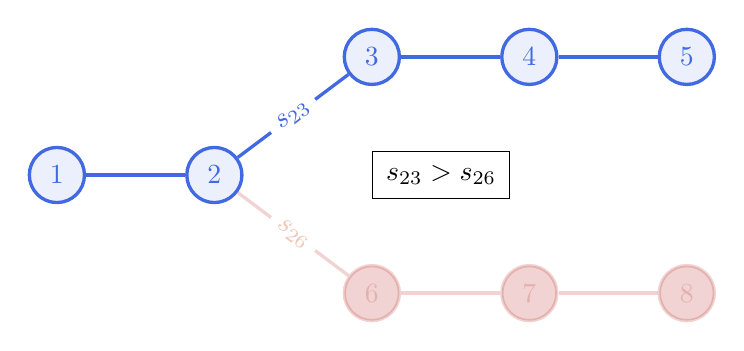
\begin{tikzpicture}
        [
            roundnode/.style={circle, text=RoyalBlue, draw=RoyalBlue!100, fill=RoyalBlue!10, very thick, minimum size=7mm},
        ]
        \node[roundnode] (1) at (0,0) {1};
        \node[roundnode] (2) at (2,0) {2};   
        \node[roundnode] (3) at (4,1.5) {3};   
        \node[roundnode] (4) at (6,1.5) {4};   
        \node[roundnode] (5) at (8,1.5) {5};
        \node[roundnode, BrickRed, opacity=0.2] (6) at (4,-1.5) {6};
        \node[roundnode, BrickRed, opacity=0.2] (7) at (6,-1.5) {7};
        \node[roundnode, BrickRed, opacity=0.2] (8) at (8,-1.5) {8};
        \node[inner sep = 5pt, draw, anchor=west] (text) at (4, 0) {$s_{23} > s_{26}$};
        \path[RoyalBlue, very thick] 
            (1) edge (2) 
            % (2) edge (3) 
            (3) edge (4) 
            (4) edge (5);
        \path[BrickRed, very thick, opacity=0.2] 
            (6) edge (7)
            (7) edge (8);
        \draw[RoyalBlue, very thick] (2) -- (3) node [midway, fill=white, sloped] {$s_{23}$};
        \draw[BrickRed, very thick, opacity=0.2] (2) -- (6) node [midway, fill=white!100, text=BrickRed!20, sloped, opacity=1] {$s_{26}$};
    \end{tikzpicture}
    \caption{An ambiguity occurs when two candidate paths have equal lengths. The path stemming from the higher edge score at the junction is selected. }
    \label{fig:walk-multi-longest}
\end{figure}
With the Walkthrough technique, the track finding part of the GNN4ITk algorithm is concluded.
The final product of graph segmentation is simple a set of track candidates.
Each candidate is a list of space points ordered by their distance from the origin. 
Equivalently, the CKF also creates a collection of track candidates, which are subjected to an ambiguity resolution step to reduce the number of shared hits and fake tracks, as described in chapter \ref{chap:atlas-reco-chain}. 
Different from GNN-built tracks, CKF tracks by construction ``live" in Athena as a link in the event reconstruction chain, and more importantly, are equipped with the track parameters. 
From an engineering point of view, it is crucial to treat GNN-built track candidates in Athena, so that they can rejoin the chain and be ready for downstream tasks.
This also enables an apple-to-apple performance comparison of both track finders in the same environment, which is presented in the next chapter.



